
%(BEGIN_QUESTION)
% Copyright 2007, Tony R. Kuphaldt, released under the Creative Commons Attribution License (v 1.0)
% This means you may do almost anything with this work of mine, so long as you give me proper credit

Examine this process trend, showing the response of the process variable to a 10\% up-and-down step change in the controller output (placed in manual mode):

$$\includegraphics[width=15.5cm]{i01724x01.eps}$$

What characteristics of the process (and its related instrumentation) can you discern from this trend?  Based on this information, do you think the process might benefit from a controller with aggressive P, I, or D action?  Explain why or why not for each action.

\vskip 20pt \vbox{\hrule \hbox{\strut \vrule{} {\bf Suggestions for Socratic discussion} \vrule} \hrule}

\begin{itemize}
\item{} One area of confusion for new students is whether any given trend graph reveals an {\it open-loop} test or a {\it closed-loop} test.  Explain how it is possible to discern the kind of test done on this process just by looking at the trend lines.
\item{} Explain why it is important to determine whether the trend graph reveals an {\it open-loop} test or a {\it closed-loop} test.  What difference does this determination make?
\item{} Suppose an inexperienced instrument technician looks at this trend and declares, ``Look, you can see that the controller here is direct-acting, because the PV and Output go in the same direction!''  Explain what is wrong with this conclusion, and how we know it is wrong from a careful inspection of the graph.
\end{itemize}

\underbar{file i01724}
%(END_QUESTION)





%(BEGIN_ANSWER)

This is a self-regulating process with about half a minute of lag time and just a bit of dead time.

\vskip 10pt

Aggressive integral action should be avoided, however some integral action will be necessary to avoid proportional-only offset.  This process is a good candidate for some derivative control action (so long as the noise is not too severe), as derivative tends to cancel out first-order lag.

%(END_ANSWER)





%(BEGIN_NOTES)

The process gain is somewhere around 0.8, which may provoke some to conclude that the controller gain must be less than 1.25 to avoid oscillation.  However, the rule of keeping loop gain less than unity may be broken if the process in question is dominated by first-order lag as this one appears to be.

First-order lag processes cannot oscillate with increasing gain, because their phase shift never exceeds 90$^{o}$.  Recall that in order to turn an amplifier into an oscillator we need to have a total gain equal to or greater than unity {\it and} 360$^{o}$ of total phase shift.  Here, a proportional controller's inherent phase shift of 180$^{o}$ plus the process's ultimate phase shift of 90$^{o}$ just doesn't add up to enough for oscillation.

%INDEX% Control, PID tuning: predicting PID requirements based on open-loop response

%(END_NOTES)


